\documentclass[11pt,a4paper]{article}
\usepackage[utf8]{inputenc}
\usepackage[margin=2.3cm]{geometry}
\usepackage{amsmath}
\usepackage{graphicx}
\usepackage{booktabs}
\usepackage{tabularx}
\usepackage{siunitx}
\usepackage[font=small,labelfont=bf]{caption}
\usepackage{subcaption}
\usepackage{float}
\usepackage{enumitem}
\usepackage{xcolor}
\usepackage[colorlinks=true,linkcolor=blue!50!black,urlcolor=blue!50!black,citecolor=blue!50!black]{hyperref}

\graphicspath{{figures/}}
\setlength{\parskip}{0.4em}
\setlength{\parindent}{0pt}

\title{DECOVALEX SAFENET: Specifications of the STIMTEC\\ Model Comparison Challenge}
\author{Olaf Kolditz\\ \small Helmholtz Centre for Environmental Research -- UFZ}
\date{20 October 2026}

\begin{document}
\maketitle

\begin{abstract}
The challenge asks every DECOVALEX SAFENET team to identify the hydraulic parameters permeability $k$ and storativity $S$ from the STIMTEC pumping tests BH~40.6 and BH~51.6, and to compare the identified values across teams and codes. The target quantity is the fluid pressure build-up in the injection interval. This report specifies data, conceptual models, meshes, parameter functions, modelling steps and requested output, and gives the reference results of the coordinating team.
\end{abstract}

%==========================================================
\section{Intention and goal of the challenge}

Modelling STIMTEC is one of three experiment-based challenges of the SAFENET task \cite{kolditz2025}. The others are the GREAT cell experiments \cite{mollaali2026} and the Thermoslip-flow cell experiments at Chongqing University. SAFENET links these laboratory tests to the STIMTEC field scale through HM+T, TM+H and THM benchmarks (Figure~\ref{fig:concept}).

This report is the specification of the STIMTEC challenge. It contains the information each team needs to parameterise its own model. As a result of the challenge, the identified hydraulic parameters ($k$, $S$) obtained by the modelling teams with their particular simulation codes will be compared.

\begin{figure}[H]
  \centering
  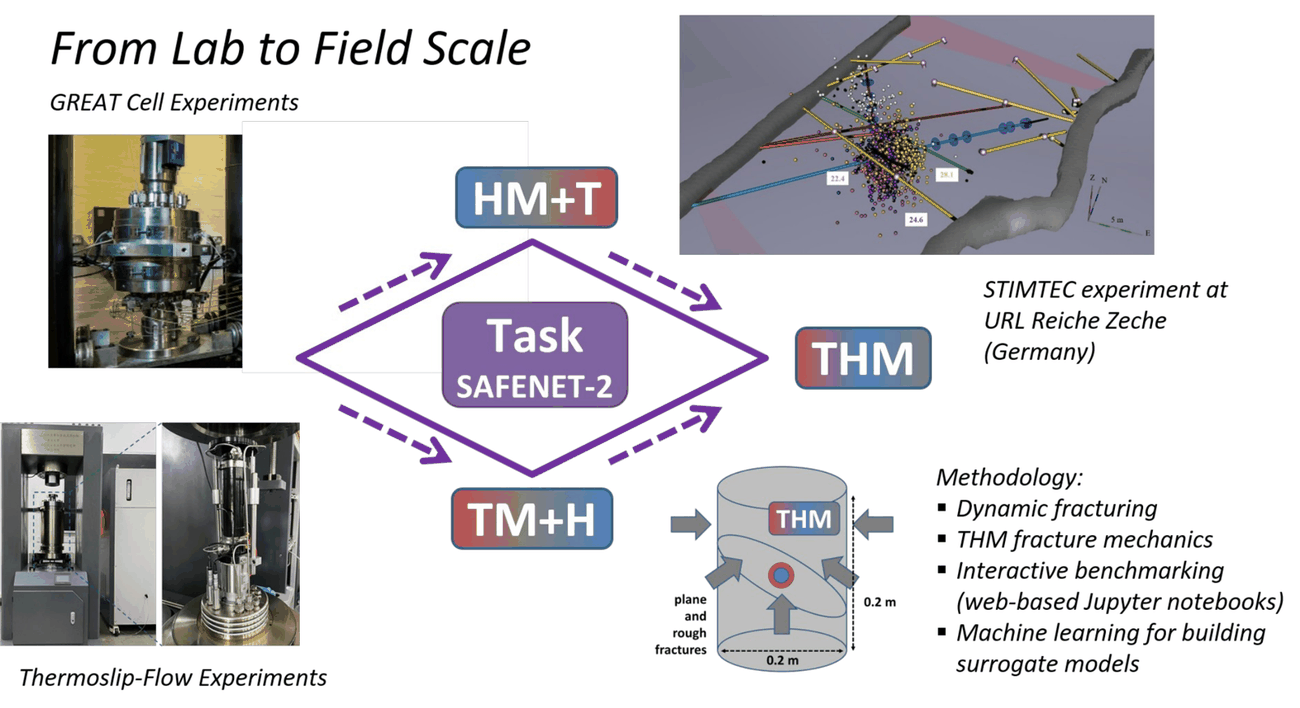
\includegraphics[width=0.9\textwidth]{s03_1.png}
  \caption{SAFENET concept -- from lab scale (GREAT cell, Thermoslip-flow) to field scale (STIMTEC, URL Reiche Zeche, Germany).}
  \label{fig:concept}
\end{figure}

The GREAT cell benchmarks set the pattern for the comparison: a sequence of cases of rising complexity, from mechanics only (M1, M3a/b) through hydro-mechanics with single and branched fractures (HM2--HM4) to thermo-hydro-mechanics (THM2--THM4) (Figure~\ref{fig:great}). The STIMTEC challenge follows the same stepwise logic: single fracture first, then fracture network.

\begin{figure}[H]
  \centering
  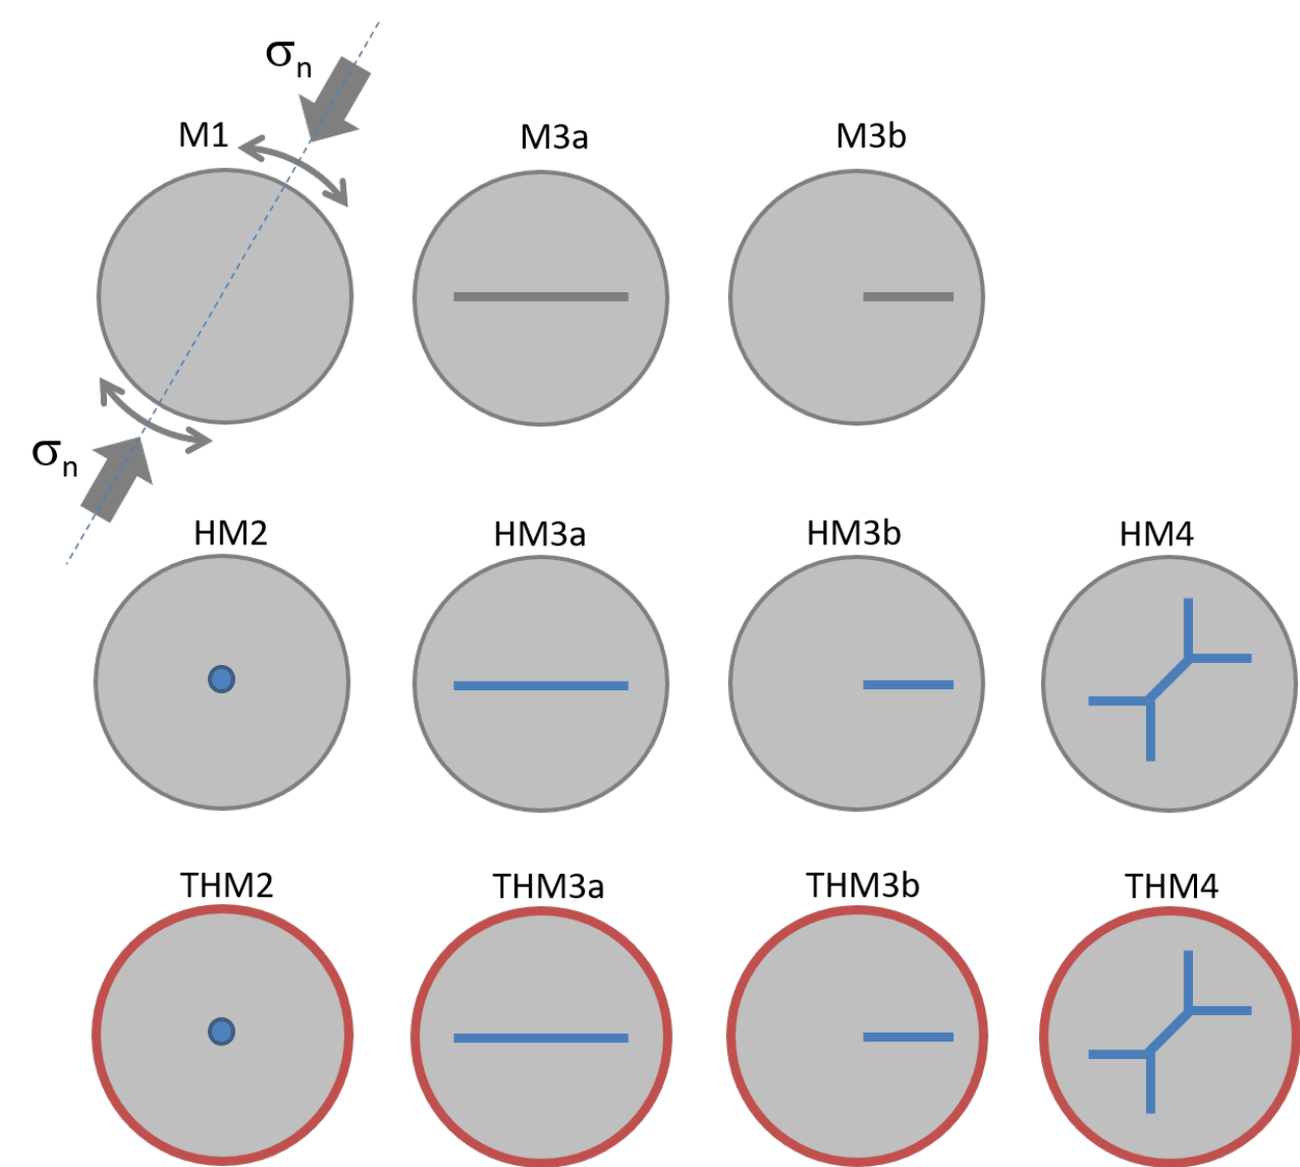
\includegraphics[width=0.5\textwidth]{s04_1.png}
  \caption{GREAT cell benchmark sequence \cite{mollaali2026}: mechanical (M), hydro-mechanical (HM) and thermo-hydro-mechanical (THM) cases.}
  \label{fig:great}
\end{figure}

%==========================================================
\section{STIMTEC experiment and data basis}

The data basis is the two step-rate pumping tests BH~51.6 and BH~40.6, conducted in borehole BH10 of the STIMTEC experiment at the underground research laboratory Reiche Zeche (Freiberg, Germany). Figure~\ref{fig:site} shows the borehole layout and the induced seismicity between the galleries; Figure~\ref{fig:data} shows the measured data.

\begin{figure}[H]
  \centering
  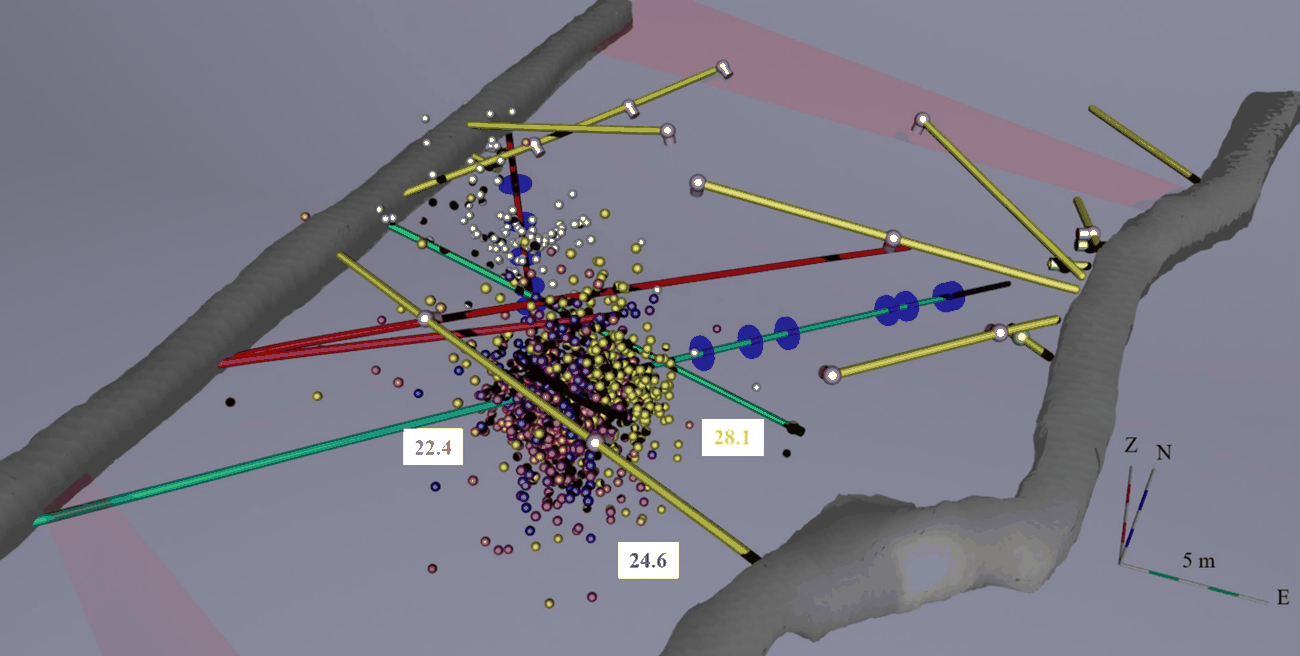
\includegraphics[width=0.85\textwidth]{s05_1.png}
  \caption{STIMTEC experiment at URL Reiche Zeche: boreholes, injection intervals and acoustic emission events between the galleries (scale bar 5\,m).}
  \label{fig:site}
\end{figure}

\begin{figure}[H]
  \centering
  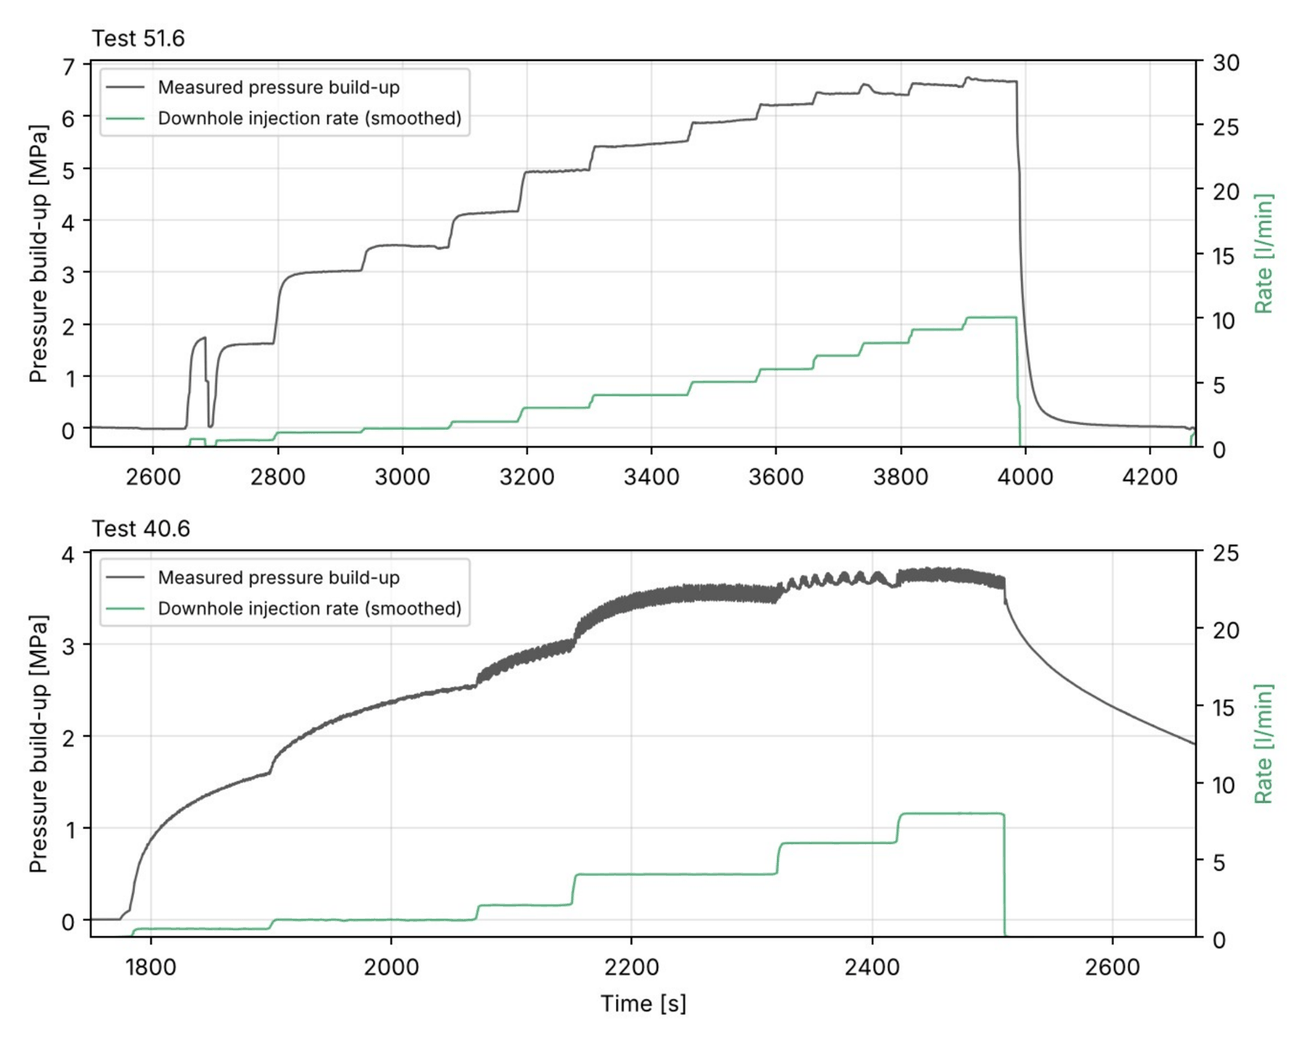
\includegraphics[width=0.72\textwidth]{s06_1.png}
  \caption{Measured pressure build-up (black) and smoothed downhole injection rate (green) for tests BH~51.6 (top) and BH~40.6 (bottom).}
  \label{fig:data}
\end{figure}

\begin{table}[H]
  \centering
  \caption{Pumping tests in BH10.}
  \begin{tabular}{lcccc}
    \toprule
    Test & Time window [s] & Rate steps & Max.\ rate [l/min] & Max.\ $\Delta p$ [MPa] \\
    \midrule
    BH 51.6 & 2500--4000 (shut-in $\approx$3990) & 15 & $\approx$10.0 & $\approx$6.8 \\
    BH 40.6 & 1750--2670 (shut-in $\approx$2510) & 7 & $\approx$8.0 & $\approx$3.8 \\
    \bottomrule
  \end{tabular}
\end{table}

Both tests show a strongly non-linear pressure--rate response: the rate rises by a factor of $\approx$15, the pressure only by a factor of $\approx$2--2.3. Each rate step reaches a pressure plateau quickly in BH~51.6, while BH~40.6 shows a slower transient rise and a slow pressure decay after shut-in.

%==========================================================
\section{Conceptual models and meshes}

Teams model the tests with a hierarchy of four conceptual models, from a single fracture to a fracture network with explicit rock matrix (Table~\ref{tab:models}, Figure~\ref{fig:approach}). SF-1 is mandatory so that all codes can be compared on a common case; the other models are optional.

\begin{table}[H]
  \centering
  \caption{Conceptual models.}
  \label{tab:models}
  \begin{tabularx}{\textwidth}{lXll}
    \toprule
    Model & Fractures & Rock matrix & Fracture--matrix exchange \\
    \midrule
    SF-1 single fracture & one, explicit (2D) & not discretised & leakage function \\
    SF-2 single fracture + matrix & one, explicit, axisymmetric & explicit & resolved \\
    DFN fracture network & field geometry, explicit & not discretised & leakage function \\
    DFNM network + matrix & field geometry, explicit & explicit & resolved \\
    \bottomrule
  \end{tabularx}
\end{table}

\begin{figure}[H]
  \centering
  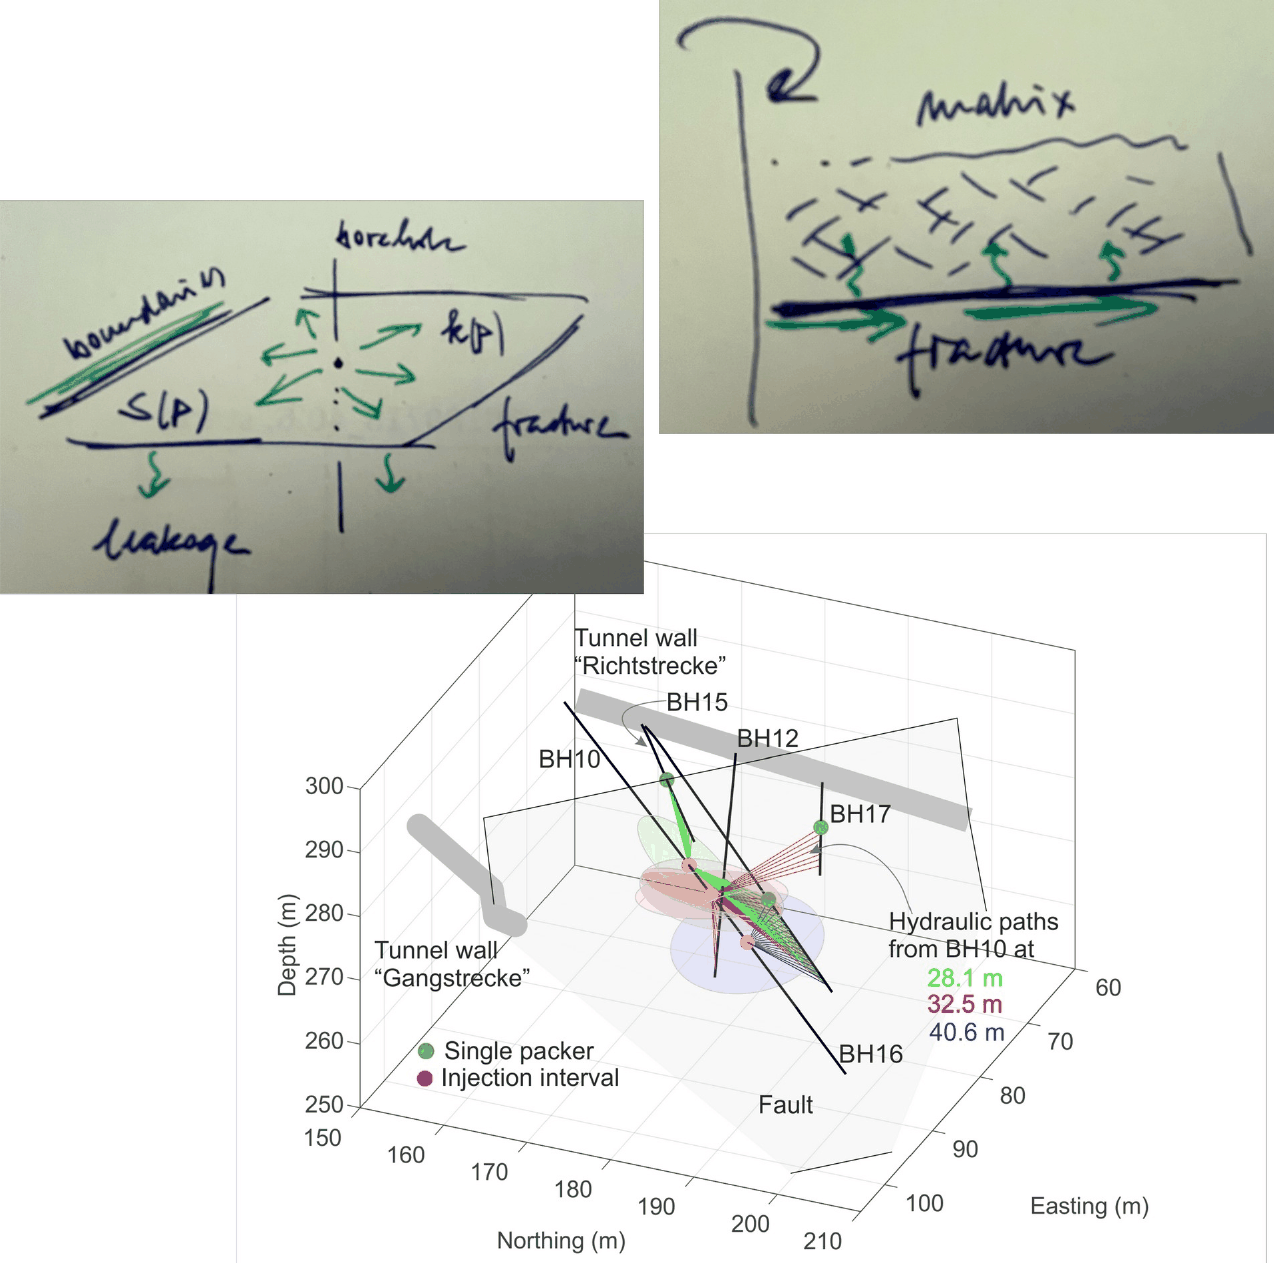
\includegraphics[width=0.6\textwidth]{s07_1.png}
  \caption{Modelling approach. Top left: single fracture with leakage functions $k(p)$, $S(p)$. Top right: axisymmetric fracture--matrix model. Bottom: fracture geometry and hydraulic paths from BH10 (28.1, 32.5, 40.6\,m) as known from the field investigation.}
  \label{fig:approach}
\end{figure}

Figure~\ref{fig:mesh} shows example finite element meshes. The single fracture reference mesh is a $100\,\text{m}\times100\,\text{m}$ square (939 nodes, 1796 triangles), refined towards the injection point \emph{well} at (0,\,0); boundary geometries are the edge \emph{right} ($x=50$\,m) and the point \emph{right\_mid} (50,\,0). The DFN mesh holds four planar elliptical fractures (1834 nodes, 3440 triangles, mean edge length 1.8\,m). BH10 intersects fracture~1 at node 270 and fracture~2 at node 271, both inside the packer interval (Table~\ref{tab:dfn}).

\begin{figure}[H]
  \centering
  \begin{subfigure}[b]{0.52\textwidth}
    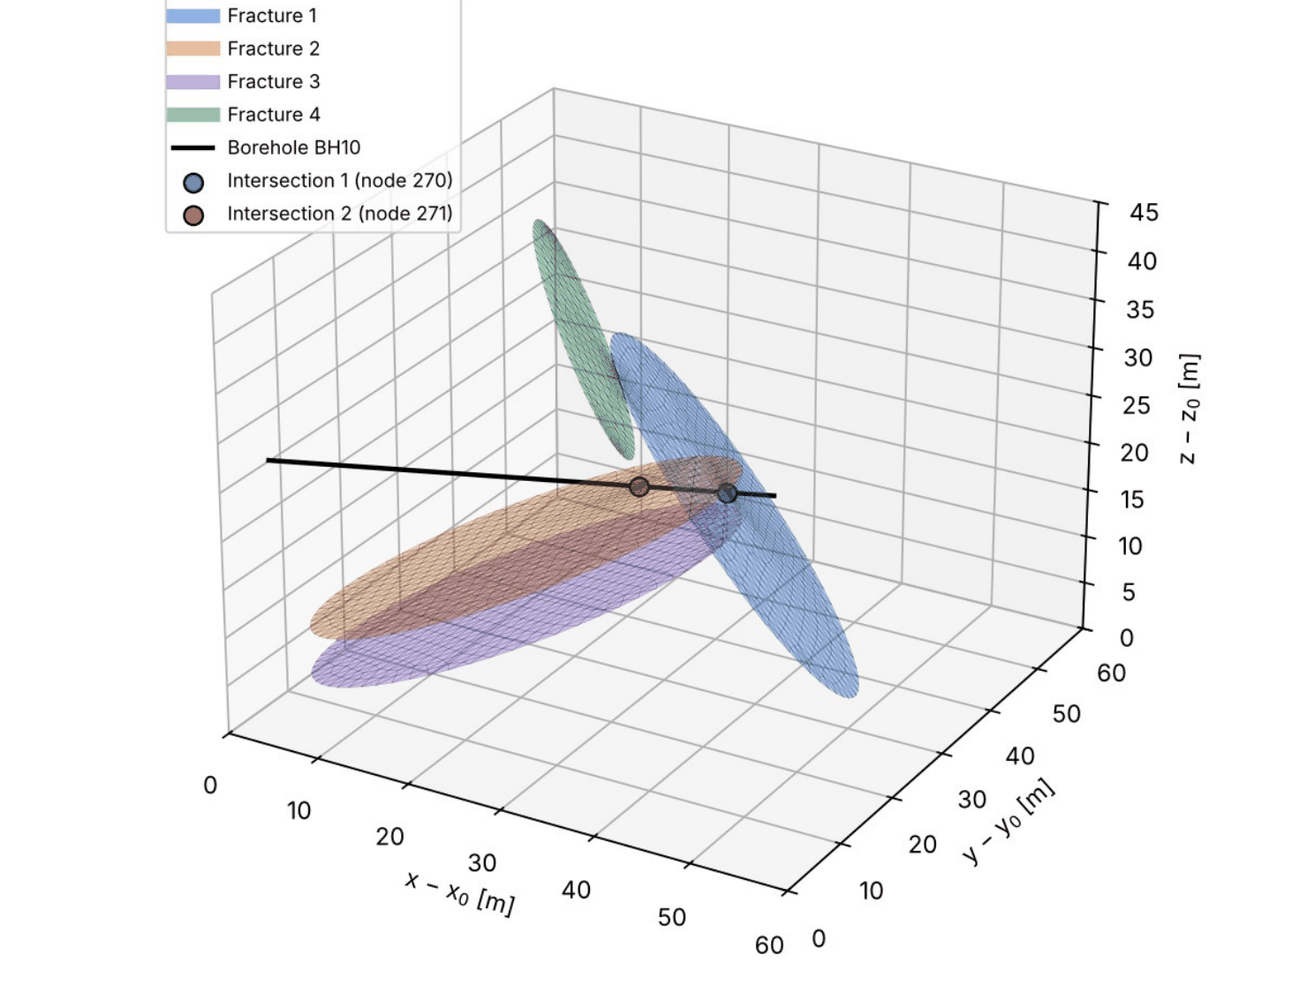
\includegraphics[width=\textwidth]{s08_1.png}
    \caption{DFN with fractures 1--4 and BH10}
  \end{subfigure}\hfill
  \begin{subfigure}[b]{0.44\textwidth}
    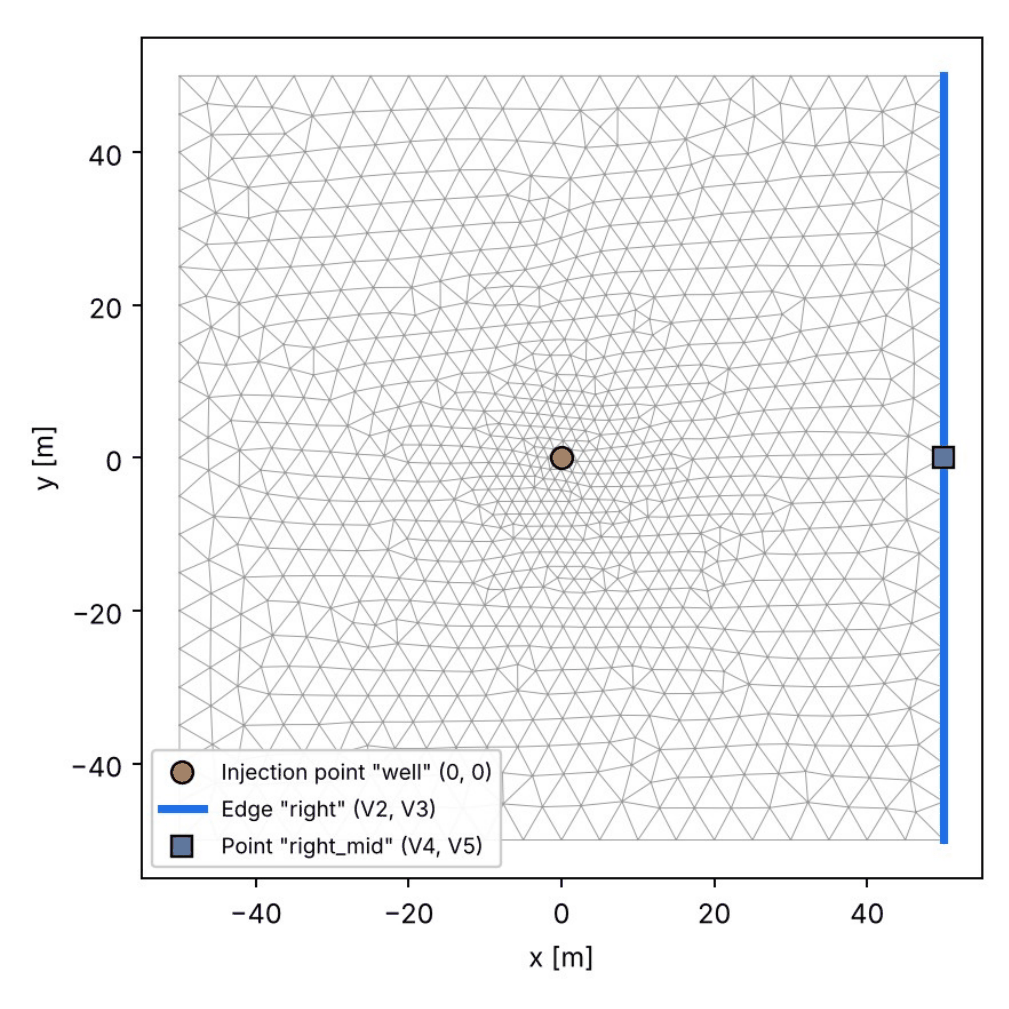
\includegraphics[width=\textwidth]{s08_2.png}
    \caption{Single fracture mesh}
  \end{subfigure}
  \caption{Example meshes. (a) DFN with borehole BH10 and its intersections (nodes 270, 271). (b) Single fracture mesh with injection point and boundary geometries.}
  \label{fig:mesh}
\end{figure}

\begin{table}[H]
  \centering
  \caption{DFN fracture geometry.}
  \label{tab:dfn}
  \begin{tabular}{cccc}
    \toprule
    Fracture & Dip direction / dip [$^\circ$] & Area [m$^2$] & Intersected by BH10 \\
    \midrule
    1 & 053 / 53 & 1599 & yes, node 270 \\
    2 & 270 / 24 & 1434 & yes, node 271 \\
    3 & 270 / 24 & 1434 & no \\
    4 & 053 / 55 & 497 & no \\
    \bottomrule
  \end{tabular}
\end{table}

%==========================================================
\section{Governing equation, parameters, initial and boundary conditions}

Flow in the fractures is single-phase liquid flow (Darcy), solved for the pressure $p$:
\begin{equation}
  S\,\frac{\partial p}{\partial t} - \nabla\cdot\left(\frac{k}{\mu}\,\nabla p\right) = Q(t).
\end{equation}
The unknowns to identify are $k$ [m$^2$] and $S$ [1/Pa]. The pumping data show that both depend on pressure, i.e.\ on the injection rate (Figure~\ref{fig:kS}). Teams therefore identify them in two forms: constant ($k$, $S$) and rate-dependent $k(t)$, $S(t)$. The reference parameterisation maps each rate step linearly between a minimum and a maximum value, which gives four unknowns:
\begin{equation}
  X(t) = X_{\min} + (X_{\max}-X_{\min})\,\frac{q(t)-q_{\min}}{q_{\max}-q_{\min}}, \qquad X\in\{k,S\}.
\end{equation}
After shut-in $X=X_{\min}$. A pressure-explicit alternative $k(p)=k_0\exp(\beta_k p)$, $S(p)=S_0\exp(\beta_S p)$ may be used as well.

\begin{figure}[H]
  \centering
  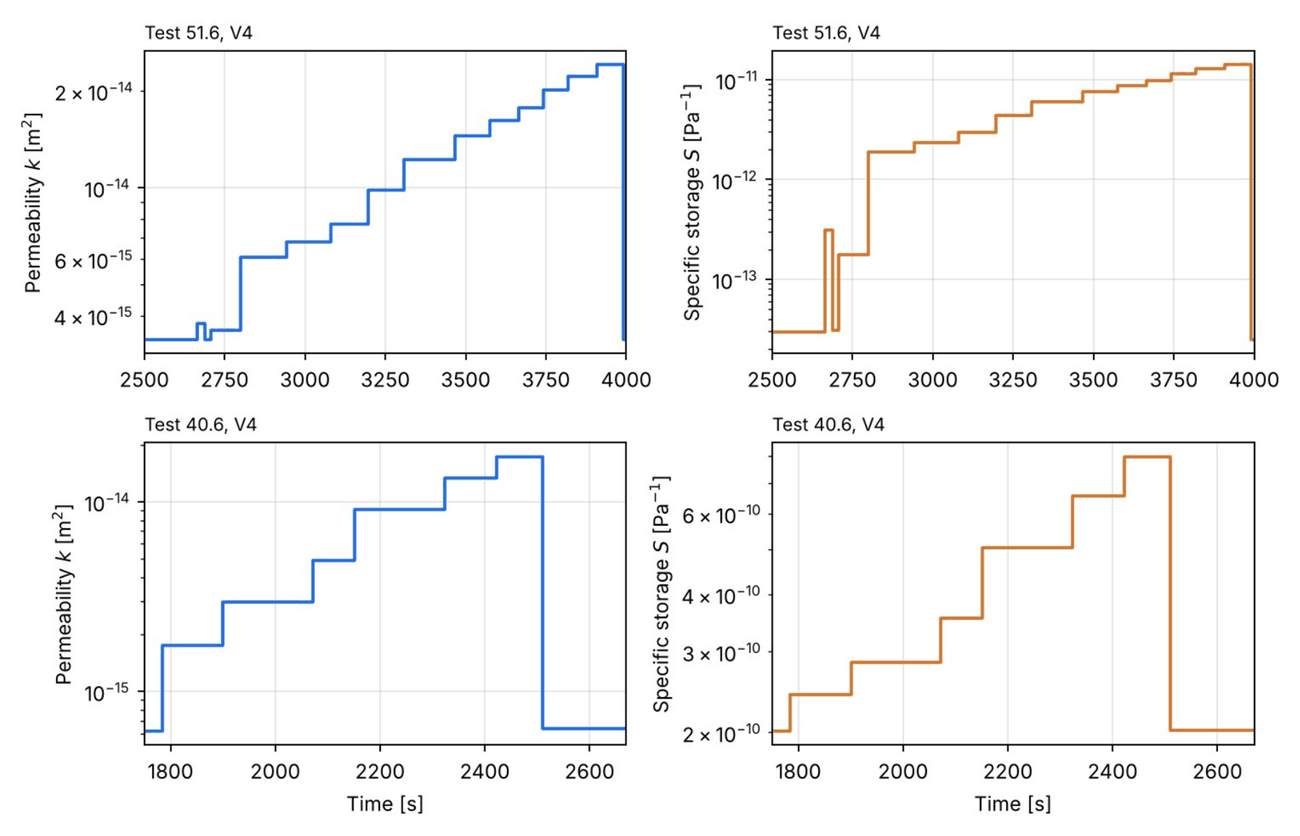
\includegraphics[width=0.75\textwidth]{s09_1.png}
  \caption{Rate-dependent permeability $k(t)$ and specific storage $S(t)$ of the single fracture model (variant V4) for tests BH~51.6 (top) and BH~40.6 (bottom).}
  \label{fig:kS}
\end{figure}

\begin{table}[H]
  \centering
  \caption{Model specification.}
  \begin{tabularx}{\textwidth}{lX}
    \toprule
    Item & Specification \\
    \midrule
    Fluid & water, $\rho=1000$\,kg/m$^3$, $\mu=1.0\cdot10^{-3}$\,Pa\,s \\
    Source term & injection rate steps from the measured downhole rate, $q$ [m$^3$/s] $=q$ [l/min]$/60000$ \\
    Initial condition & $p_0=1$\,MPa (single fracture) or hydrostatic (DFN); compare build-up $\Delta p=p-p_0$ \\
    BC, single fracture & Dirichlet $p_0$ on edge \emph{right} (V3) or point \emph{right\_mid} (V4); closed edges for V1 \\
    BC, DFN & Dirichlet $p_0$ on all fracture rim nodes \\
    Fracture thickness & unit thickness 1\,m (single fracture); aperture 1\,m in DFN for consistency \\
    Rate partitioning, DFN & fixed share of the rate to fractures 1 and 2 (50/50 or calibrated) \\
    Time stepping & fixed $\Delta t=10$\,s (BH~51.6), 5\,s (BH~40.6) \\
    Measured baseline & subtract median before pumping: 0.150\,MPa (51.6), 0.087\,MPa (40.6) \\
    \bottomrule
  \end{tabularx}
\end{table}

%==========================================================
\section{Modelling steps and reference results}

Each team runs the steps below for both tests; Steps 1--2 (SF-1) are mandatory, Steps 3--5 optional. Teams report the identified $k$ and $S$ per step. The reference results of the coordinating team (OpenGeoSys 6.5, LiquidFlow) are given in Figures~\ref{fig:res51}--\ref{fig:dfnsplit} and Table~\ref{tab:ref} as orientation.

\begin{enumerate}[leftmargin=*,itemsep=2pt]
  \item \textbf{Step 1 -- constant parameters (V1/V2):} single fracture, constant $k$ and $S$, closed or Dirichlet boundary.
  \item \textbf{Step 2 -- rate-dependent parameters (V3/V4):} single fracture, $k(t)$, $S(t)$ coupled to the injection rate; edge or point boundary.
  \item \textbf{Step 3 -- pressure-dependent parameters (V5):} single fracture, $k(p)$, $S(p)$ by exponential functions (optional).
  \item \textbf{Step 4 -- DFN:} constant and rate-dependent $k$, $S$ on the four-fracture network, with rate partitioning between fractures 1 and 2 (optional).
  \item \textbf{Step 5 -- DFNM:} fracture network with explicit matrix (optional, open).
\end{enumerate}

\begin{figure}[H]
  \centering
  \begin{subfigure}[t]{0.49\textwidth}
    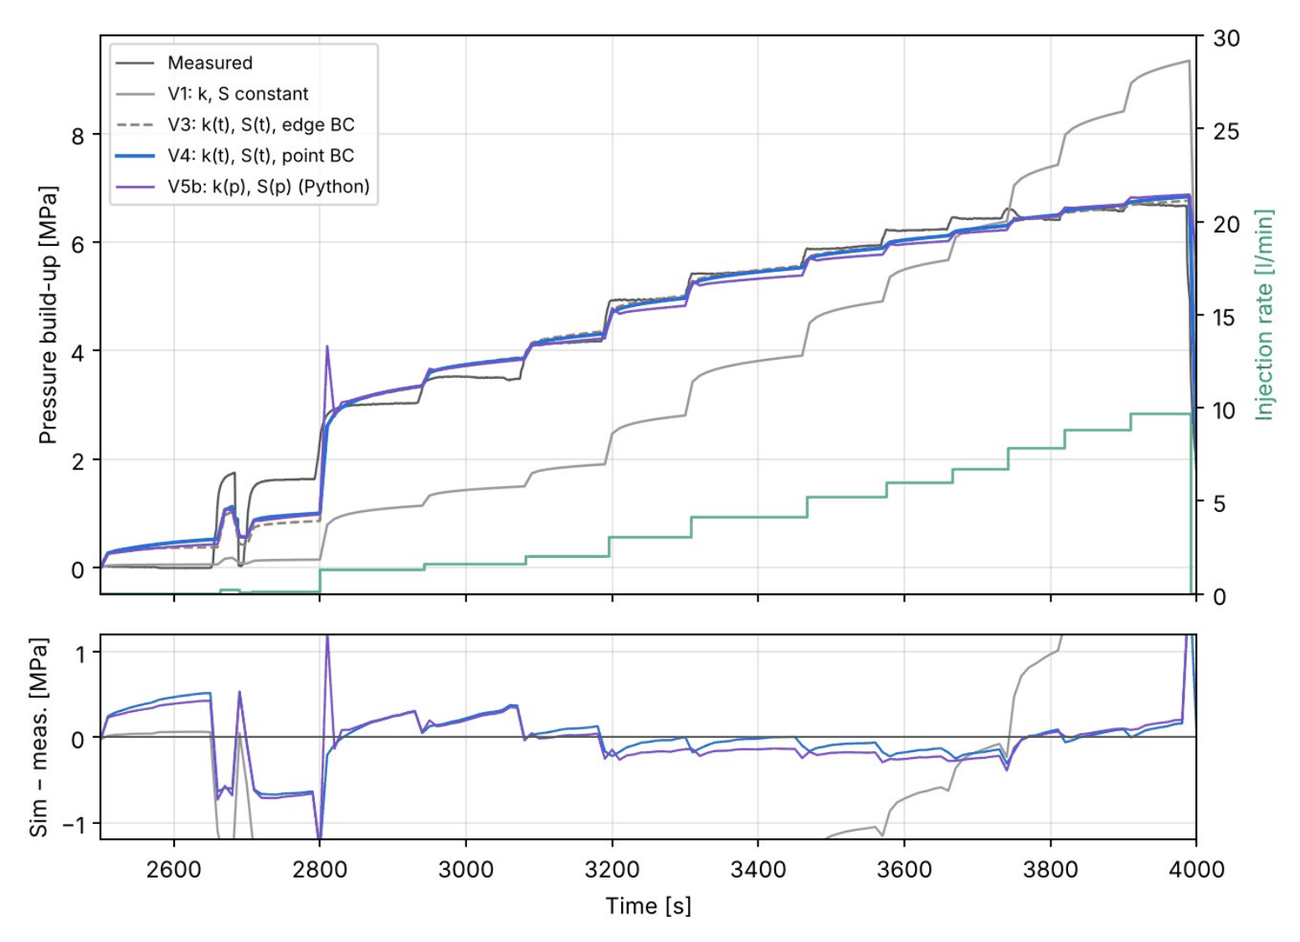
\includegraphics[width=\textwidth]{s10_1.png}
    \caption{Test BH 51.6}
    \label{fig:res51}
  \end{subfigure}\hfill
  \begin{subfigure}[t]{0.49\textwidth}
    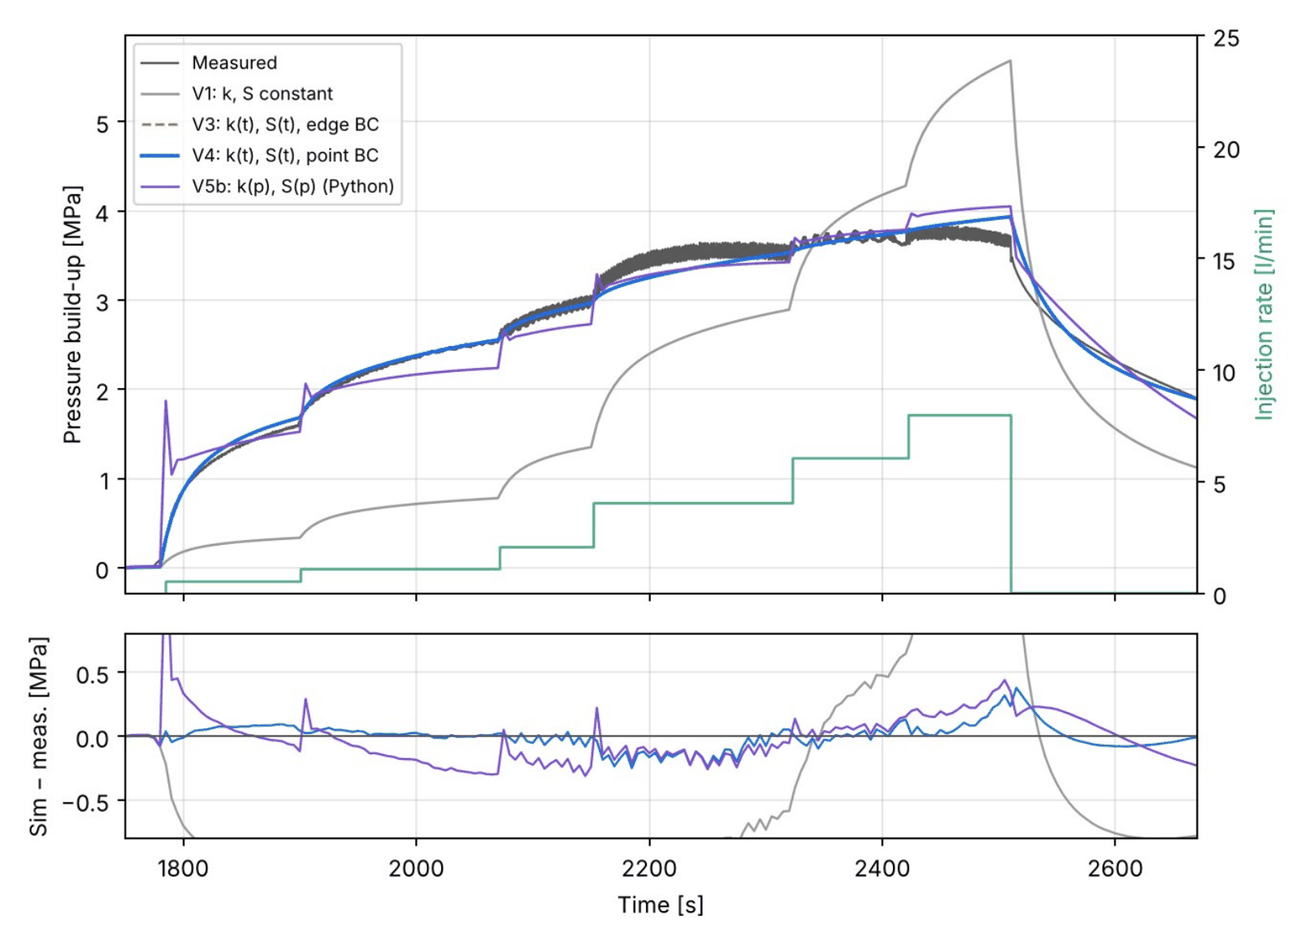
\includegraphics[width=\textwidth]{s11_1.png}
    \caption{Test BH 40.6}
    \label{fig:res40}
  \end{subfigure}
  \caption{Single fracture model: measured vs.\ simulated pressure build-up for variants V1, V3, V4, V5b (top) and residuals (bottom).}
\end{figure}

\begin{figure}[H]
  \centering
  \begin{subfigure}[t]{0.49\textwidth}
    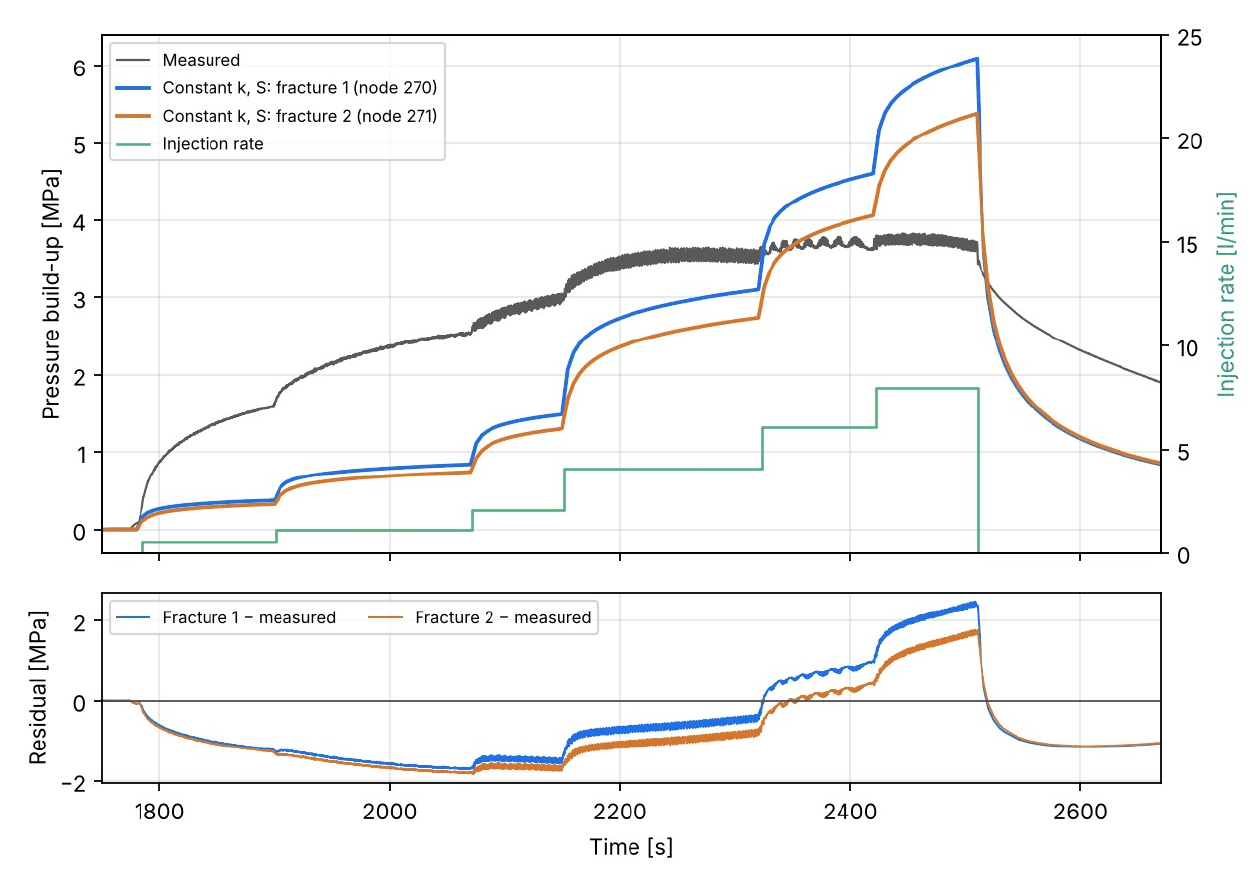
\includegraphics[width=\textwidth]{s12_1.png}
    \caption{Constant $k$, $S$}
    \label{fig:dfnconst}
  \end{subfigure}\hfill
  \begin{subfigure}[t]{0.49\textwidth}
    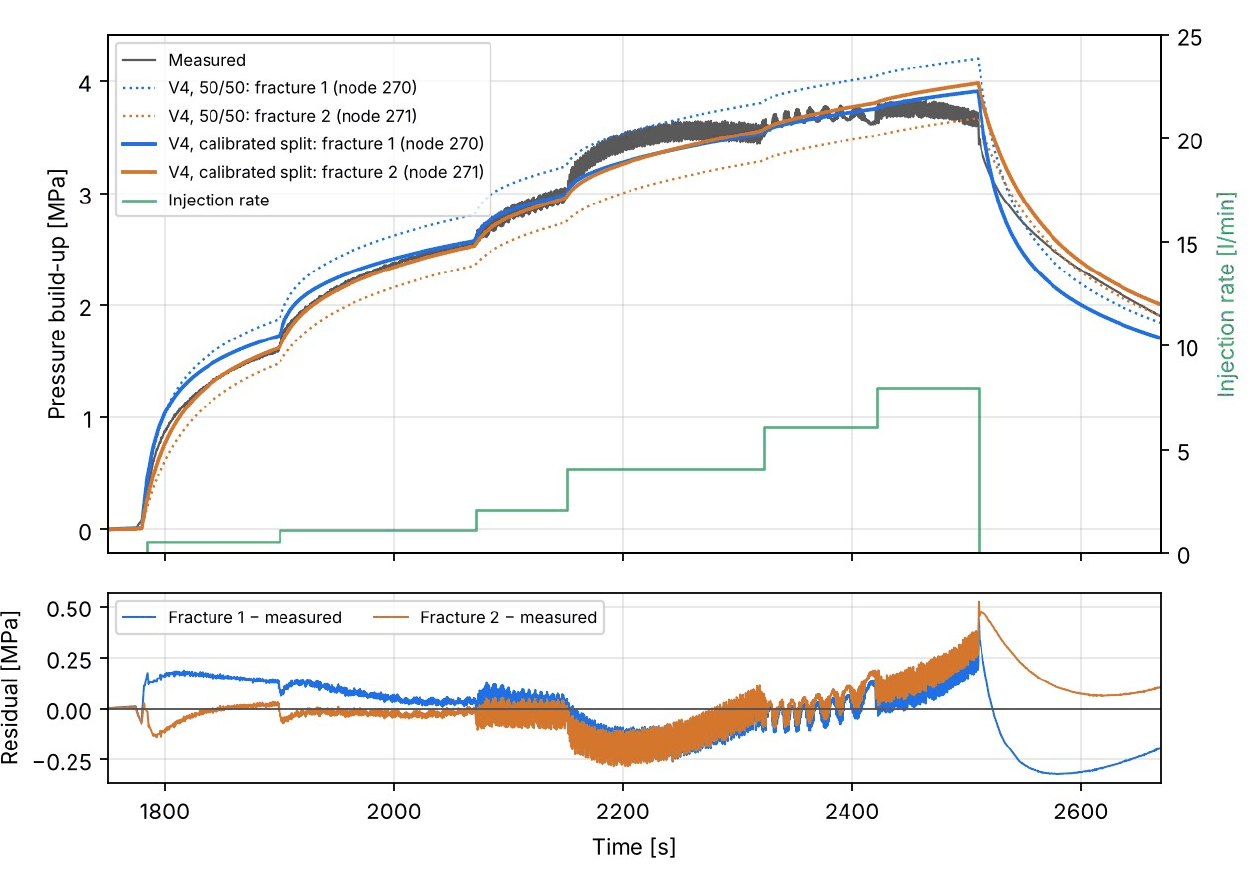
\includegraphics[width=\textwidth]{s12_2.png}
    \caption{Rate-dependent $k$, $S$ and rate partitioning}
    \label{fig:dfnsplit}
  \end{subfigure}
  \caption{DFN model, test BH~40.6: pressure at fracture~1 (node 270) and fracture~2 (node 271) with residuals. (b) compares 50/50 and calibrated rate partitioning.}
\end{figure}

\begin{table}[H]
  \centering
  \caption{Reference results of the coordinating team (OpenGeoSys).}
  \label{tab:ref}
  \footnotesize\setlength{\tabcolsep}{4pt}
  \begin{tabular}{llllc}
    \toprule
    Model / variant & Test & $k$ [m$^2$] & $S$ [1/Pa] & RMSE [MPa] \\
    \midrule
    SF V1 constant & 51.6 & 1.41e-14 & 1.42e-11 & 1.69 \\
    SF V4 $k(t)$, $S(t)$ & 51.6 & 3.37e-15 \ldots\ 2.41e-14 & 2.48e-14 \ldots\ 1.41e-11 & 0.32 \\
    SF V1 constant & 40.6 & 9.15e-15 & 1.08e-9 & 1.16 \\
    SF V4 $k(t)$, $S(t)$ & 40.6 & 6.16e-16 \ldots\ 1.73e-14 & 2.01e-10 \ldots\ 7.98e-10 & 0.10 \\
    SF V5b $k(p)$, $S(p)$ & 40.6 & $k_0$ 3.68e-15, $\beta_k$ 1.06/MPa & $S_0$ 4.73e-14, $\beta_S$ 0.79/MPa & 0.21 \\
    DFN constant & 40.6 & 6.12e-15 & 3.98e-10 & 1.24 \\
    DFN $k(t)$, $S(t)$, split 46.5/53.5\,\% & 40.6 & 3.40e-16 \ldots\ 9.06e-15 & 2.50e-10 \ldots\ 9.15e-10 & 0.12 \\
    \bottomrule
  \end{tabular}
\end{table}

Constant parameters cannot reproduce the data (RMSE $>1$\,MPa). Coupling $k$ and $S$ to the rate cuts the error by a factor of 5 (51.6) to 12 (40.6); permeability then rises with rate by a factor of $\approx$7 (51.6) and $\approx$28 (40.6), consistent with fracture opening.

%==========================================================
\section{Data provided, requested output and comparison metrics}

The main comparison quantity is the set of identified hydraulic parameters ($k$, $S$) per team, code, model and test. The pressure fit is the quality measure behind each set.

\textbf{Provided to all teams} (GitHub repository, data download): experimental data of the BH~40.6 and BH~51.6 pumping tests (xlsx, png); DFN model (vtu); DFNM model (vtu); OpenGeoSys projects of the reference models.

\begin{table}[H]
  \centering
  \caption{Deliverables requested from each team (upload by institution).}
  \begin{tabularx}{\textwidth}{lXl}
    \toprule
    Deliverable & Content & Format \\
    \midrule
    Identified parameters & $k$, $S$ (constant) and $k_{\min}/k_{\max}$, $S_{\min}/S_{\max}$ (rate-dependent) per model and test; DFN rate split & csv/xlsx \\
    Pressure time series & simulated $\Delta p$ at the injection point (SF) or nodes 270/271 (DFN) at the measurement times & csv \\
    Fit quality & RMSE of $\Delta p$ over the test window, including shut-in decay & value per run \\
    Model description & code, element type, mesh, time stepping, fluid properties, BCs, optimisation method & short text \\
    \bottomrule
  \end{tabularx}
\end{table}

The metric is the RMSE of the pressure build-up against the baseline-corrected measurement over 2500--4000\,s (BH~51.6) and 1750--2670\,s (BH~40.6). For the DFN, the RMSE is evaluated at both intersection nodes individually, since both lie in the same packer interval.

%==========================================================
\section{Summary and outlook}

The STIMTEC challenge compares hydraulic parameters identified by different teams and codes on the same field data, two step-rate tests in BH10. The reference results show that rate-dependent $k$ and $S$ are needed to fit the data, and that the DFN gives parameters close to the single fracture model once the rate is split between the two intersected fractures.

Open points for the teams: the fixed rate split cannot keep equal pressure at both intersections over the whole test; a coupled borehole element (common interval pressure) or per-fracture parameters are the natural next step. The DFNM model and coupled HM effects are left for a later phase.

\begin{thebibliography}{9}
\bibitem{kolditz2025} Kolditz, O. et al. (2025): DECOVALEX SAFENET task. \emph{Safety of Nuclear Waste Disposal} 3, 15. \url{https://doi.org/10.5194/sand-3-15-2025}
\bibitem{mollaali2026} Mollaali, M., Wang, W., You, T., Nagel, T., Fraser-Harris, A., McDermott, C., Kolditz, O. (2026): Numerical benchmarking of GREAT cell experiments: Poly-axial stress effects on fluid flow in fractured rock. \emph{Journal of Rock Mechanics and Geotechnical Engineering}. \url{https://doi.org/10.1016/j.jrmge.2026.03.060}
\end{thebibliography}

\end{document}
